\chapter{基于三维体素泛洪与线性拟合的三维树木骨架抽取}
\label{sec:sklextract}
在获取了精确的点云模型之后,出于后续轻量化的考虑,需要将模型的存储方式由
密集的点云转化为逻辑的父子结构。用树形的数据结构来表达现实的树结构,这是很
自然的想法,相对于面片结构,树形结构也是一种更为轻量化的存储方式。每个节点表示
树枝的起点,存储着该节点的空间位置,半径和该节点的父子枝信息以及兄弟信息。一个
节点和它的一个子节点形成一个空间线段,若干空间线段组成一条连续的树枝。

本文从树的生长规律入手,从根节点往子节点生长。生长的依据则为当前节点所在邻域
内的空间点云分布,节点邻域大小由步长来控制,步长会探索式地递增,直到达到了增长的阈值,
邻域大小才确定下来。然后从其点云分布拟合出各个分支的方向,从而生长出新的子节点,
并递归地生长下去直到点云的边界。

\section{点云体素化}
前面三维重建步骤得到的结果是一个点云模型,该模型中的点数量庞大,不适于后续的
邻域搜索,因此我们需要对点云进行体素化处理。所谓体素化,就是将离散的点的数据
组织形式转化为连续的体素的组织形式。它主要分为三步:\\

\begin{itemize}
	\item \textbf{求得点云包围盒}: 即找到包围点云模型中所有点的最小的长方体。如图
		\ref{fig:voxel}(a)。
	\item \textbf{包围盒空间分块}: 根据上一步得到长方体,进行空间分块,每个分块
		为一个小的立方体,即体素。如图\ref{fig:voxel}(b)。
	\item \textbf{点云索引}: 对于每一个非空的体素,进行点云的索引。如图\ref{fig:voxel}(c)。
\end{itemize}

\begin{figure}[H]
	\centering
	\subfloat[求得点云包围盒]{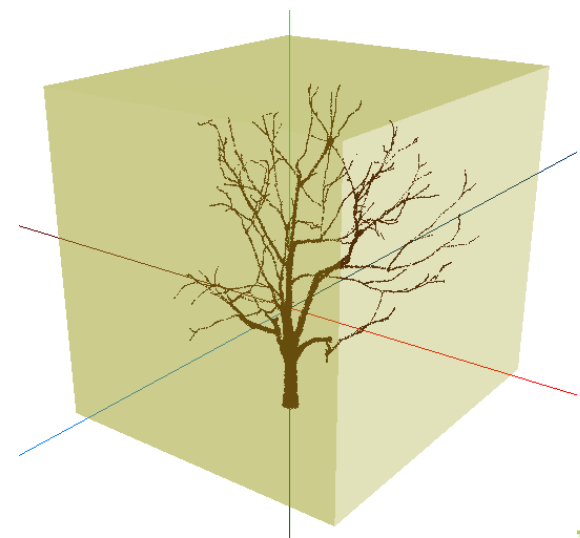
\includegraphics[width=0.3\linewidth]{box.png}}\hfill
	\subfloat[包围盒空间分块]{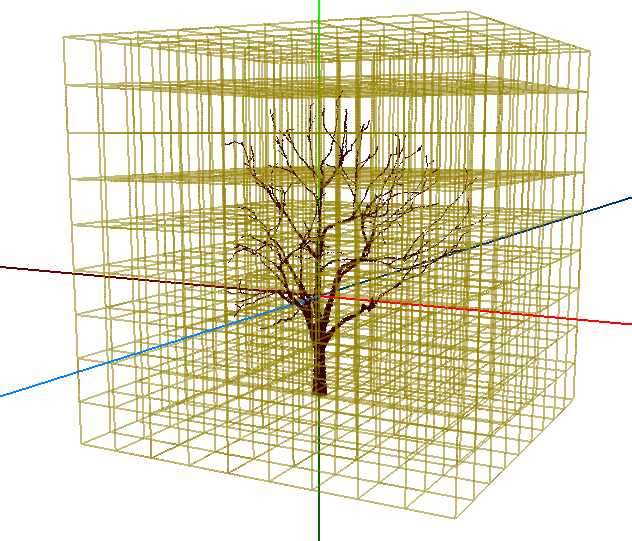
\includegraphics[width=0.3\linewidth]{voxel.png}}\hfill
	\subfloat[点云索引]{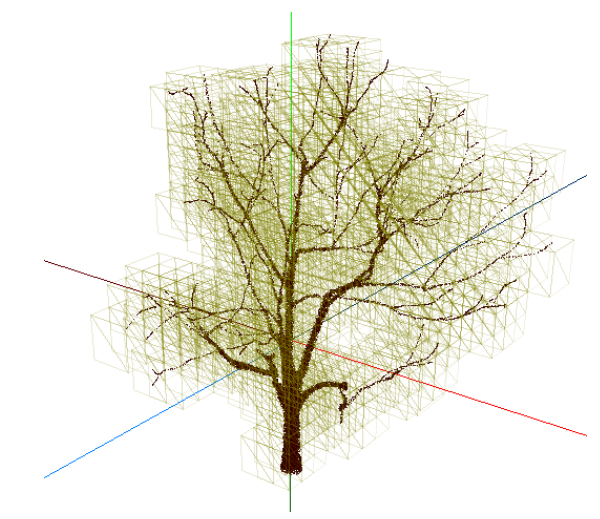
\includegraphics[width=0.3\linewidth]{index.png}}
	\caption{点云体素化}
	\label{fig:voxel}
\end{figure}

在将点云模型转化为体素模型以后,对于点云的邻域搜索便转化为了对于空间临近体素的
搜索,体素的位置就反映了点集的位置,因此不用每次搜索都遍历整个点云,而是只用将
步长范围体素中的点集遍历即可。由于体素是我们处理的基本单位,所以体素的大小也
直接决定了体素模型的精度,因此,在确保非空体素的空间连续性和效率允许的基础上,
本文建议让体素尽可能的小,以保证模型的精度。将点云模型转换为体素模型的伪代码
在算法\ref{alg:voxel}中给出。

\begin{algorithm}[H]
	\caption{点云模型体素化}
	\label{alg:voxel}
	\begin{algorithmic}[1] 
	\Require 点云模型$M$
	\Require 体素维度$d$
	\Ensure 三维体素数组$\mathbb{V}[1..d,1..d,1..d]$
	\State 初始化点云边界值$X_{max}=Y_{max}=Z_{max}=MIN\uline\quad FLOAT,X_{min}=Y_{min}=Z_{min}=MAX\uline\quad FLOAT$
	\ForAll{空间点$P(P_x,P_y,P_z) \in M$}
		\State $CheckBoundary(P)$
	\EndFor
\ForAll{空间点$P(P_x,P_y,P_z) \in M$}
\State $V_x = \frac{P_x-X_{min}}{X_{max}-X_{min}}\cdot d$
\State $V_y = \frac{P_y-Y_{min}}{Y_{max}-Y_{min}}\cdot d$
\State $V_z = \frac{P_z-Z_{min}}{Z_{max}-Z_{min}}\cdot d$
\State $\mathbb{V}[V_x, V_y, V_z] = \mathbb{V}[V_x, V_y, V_z] \bigcup \{P\} $
	\EndFor
\end{algorithmic}
\end{algorithm}

\section{三维体素泛洪确定邻域范围}
在确定了三维体素模型以后,便需要从根到叶,自底向上地对树的骨架结构进行生长。
生长的依据是已经得到的体素模型,将体素模型中点的分布作用于骨架的分支,便可以
张成骨架模型。

具体方法是将根节点置为当前节点,对其进行三维泛洪,首先对其相邻的26个体素进行泛洪,若
体素不为空,则将其加入邻域范围,若为空,则停止向该方向进行迭代。同时将加入邻域
范围的体素置为无效,表示其已经参与了泛洪,不再参与骨架的重建,这样不仅可以对算法
的结束有一个很好的约束条件,同时也可以减少重复处理的次数,加快算法的完成。然后进行下一次迭代,
对新加入的体素进行26方向的泛洪,并把有效的体素加入到邻域范围。接着比较两次迭代
体素增加的比例,如果低于设置的阈值,则停止迭代,当前的邻域范围即为三维泛洪得到
的当前节点的邻域范围。

图\ref{fig:3dfld}展示了三维体素泛洪确定邻域的步骤,三张图都延空间z轴正向投影到2D平面。
\ref{fig:3dfld}(a)为其初始状态,
即邻域范围为当前体素。其中橙色的区域表示邻域范围,蓝色的区域表示未探索区域,灰色区域
表示空的体素,而绿色区域表示已经在之前的枝干邻域。\ref{fig:3dfld}(b)表示体素泛洪经过
一次迭代以后的状态,因为体素泛洪只会对与当前邻域范围相邻的未探索区域(蓝色方块)进行扩展,
所以\ref{fig:3dfld}(a)只会向黄色箭头指向的体素进行扩展,从而得到\ref{fig:3dfld}(b)。在得到
新的邻域后,首先会计算所新增的点的数量与之前的数量的比值有没有低于阈值,如果低于阈值,则停止
邻域的扩张。最后将得到\ref{fig:3dfld}(c)中的邻域范围。

\begin{figure}[H]
	\centering
	\subfloat[初始状态(邻域范围为1个体素)]{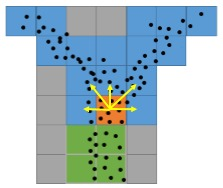
\includegraphics[height=3cm]{fld1.jpg}}\hspace{4em}
	\subfloat[第一次泛洪迭代(邻域范围为6个体素)]{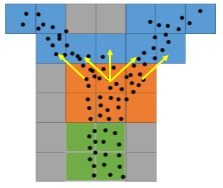
\includegraphics[height=3cm]{fld2.jpg}}\hspace{4em}
	\subfloat[第二次泛洪迭代(邻域范围为11个体素)]{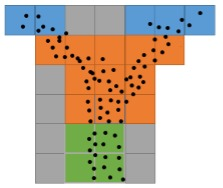
\includegraphics[height=3cm]{fld3.jpg}}
	\caption{单个体素泛洪示意图}
	\label{fig:3dfld}
\end{figure}

由于树木有多个节点,所以确定节点间的泛洪顺序十分重要。因为泛洪算法对泛洪过的区域不再进行泛洪,因此
需要将各个节点之间的相互影响降到最低。本文通过广度优先的方法,按层级对体素进行泛洪,这样就避免了子
节点的泛洪影响到叔父节点的泛洪。同时,对于同一层级的体素,将其视为多个种子点,并采取并发的泛洪,
也就是同时对它们进行泛洪,这样既提高了泛洪的效率,也使得同层级间的体素之间的影响降到最小。

图\ref{fig:flood}给出了多种子点并发泛洪确定邻域的示意图。其中蓝色方块为未泛洪体素,着红色的方块表示
已泛洪体素,橙色的小球为当前的种子点。由图可见,当前的种子点为树木的相同层级上的节点,即广度优先的
并发泛洪。

\begin{figure}[H]
	\centering
	\subfloat[步骤1]{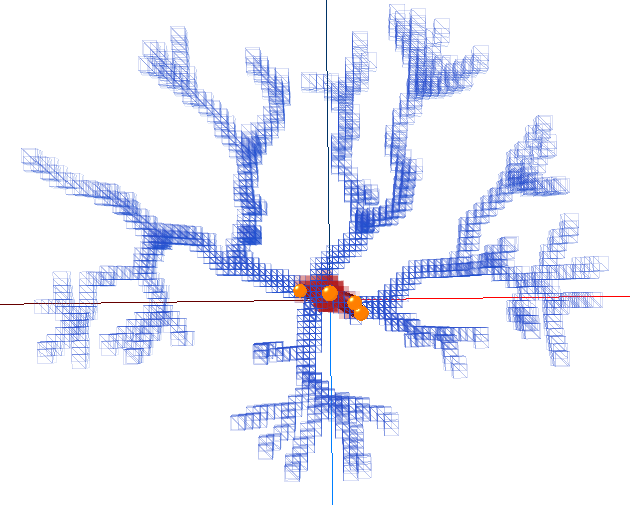
\includegraphics[width=0.4\linewidth]{seed1.png}}\hfill
	\subfloat[步骤2]{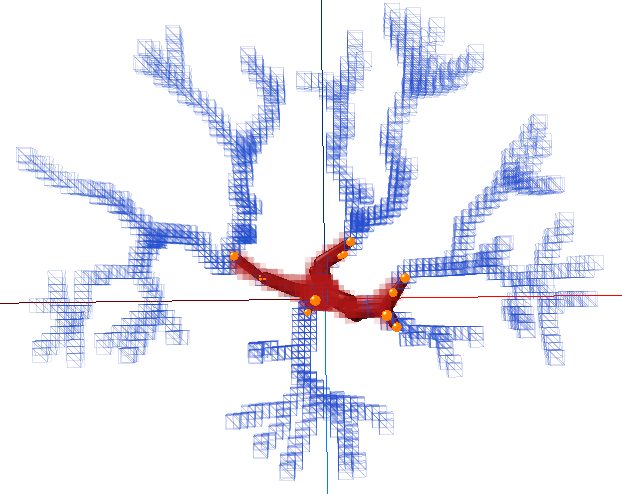
\includegraphics[width=0.4\linewidth]{seed2.png}}\hfill
	\subfloat[步骤3]{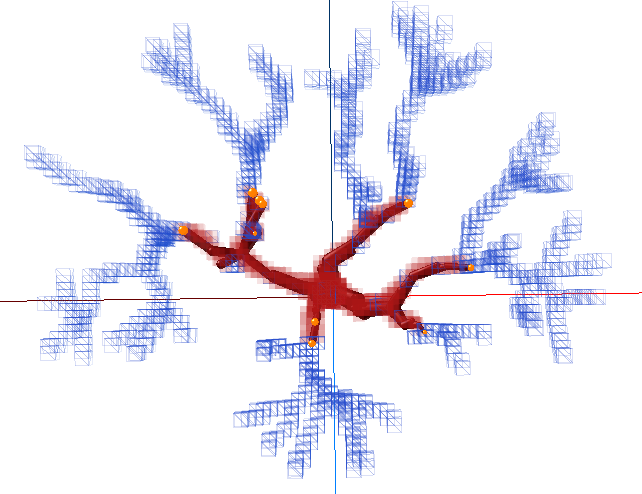
\includegraphics[width=0.4\linewidth]{seed3.png}}\hfill
	\subfloat[步骤4]{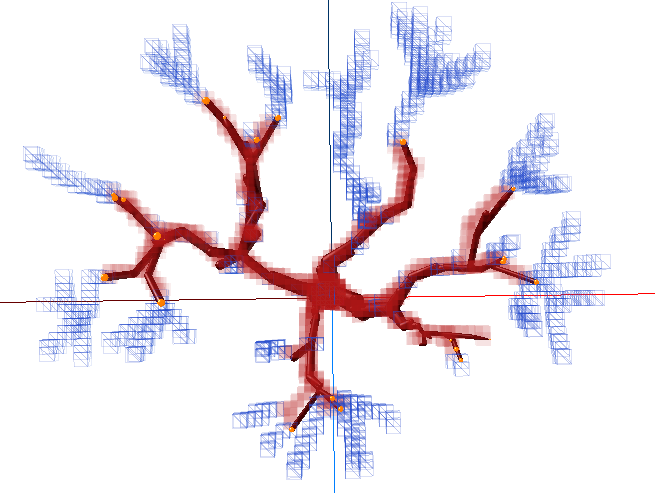
\includegraphics[width=0.4\linewidth]{seed4.png}}\hfill
	\caption{多种子点并发泛洪示意图}
	\label{fig:flood}
\end{figure}

多种子点并发体素泛洪确定邻域范围算法的伪代码在算法\ref{alg:3dfld}中给出。
\begin{algorithm}[H] 
	\caption{多种子点并发泛洪邻域探索算法}
	\label{alg:3dfld}
	\begin{algorithmic}[1]
		\Require 当前层级体素集$\mathbb{C}$,三维体素数组$\mathbb{V}[1..d,1..d,1..d]$,
		泛洪方向数组$\mathbb{D}[1..26]$,邻域范围增长比例阈值$\lambda$,最大迭代次数$num$
		\Ensure	邻域范围内体素集合$\mathbb{S}$
		\State 当前层级体素数目$n$ = $\mathbb{C}$.Count
		\State 初始化前一次泛洪体素数目数组$\mathbb{P}[1,..,n]$
		\For{i = 1 \textbf{to} $num$}
		\State 体素索引$j = 0$
		\ForAll{体素$voxel \in \mathbb{C}$}
		\State $j++$
		\State 临时体素数组$\mathbb{T}$
		\ForAll{泛洪方向$Direction \in \mathbb{D}$}
			\State $NewIndex = voxel.Index + Direction$
			\State $NewVoxel = \mathbb{V}[NewIndex.x,NewIndex.y,NewIndex.z]$
			\If{$NewVoxel$非空$\bigcap NewVoxel$有效}
				\State $\mathbb{T}.AddVoxel(NewVoxel)$
			\EndIf
		\EndFor
		\State 体素增长比例$\mu=\frac{\mathbb{T}.Count}{\mathbb{P}[j]}$
		\If{$\mu > \lambda$}
			\ForAll{$voxel \in \mathbb{T}$}
				\State S.AddVoxel(voxel)
			\EndFor
		\EndIf
		\EndFor
		\EndFor
		\State \Return $\mathbb{S}$
	\end{algorithmic}
\end{algorithm}

\section{最小二乘法线性拟合确定分支方向}
\label{subsec:leastsquares}
当得到邻域范围以后,便得到了邻域内体素在基于当前节点26个方向上的密度分布,而
每个体素内又包含着若干的点,因此等于是得到了在当前节点邻域内的点云分布情况。
接下来的工作就是怎样从各个方向的点云的分布情况抽取出核心的骨架。本文应用线性
拟合的方法来从密集的点中抽取出一条直线,作为该部分的骨架方向。

该方法首先要剔除掉那些点云密度很小的方向,以免每个节点都朝各个方向长出一些
细碎的枝条。因为这些细碎的枝条就算在此步中不剔除,到后续的轻量化的时候也不容许
它们的存在。

然后对于剩下的若干方向$d_1,d_2...d_k$,每个方向都对应着树木的一个骨架。在处理
某个方向$d_i$时,将其包含的体素中的所有点抽取出来,得到一个密集的点集$S_i$。
然后采用待定方程的办法,设直线方程为:
\begin{equation}
	\mathbf{x} = \mathbf{x_0} + \mathbf{d}t,\quad(t \in [0,\infty))
\end{equation}

其中$\mathbf{x_0}$是当前节点的坐标,$\mathbf{d}$是待拟合的直线方向。我们假设
点集$S_i$中的点$P_1,P_2,...P_m$都在直线上,则可以得到以下方程组:\\

\begin{equation} \label{eq:line}
	\left\{ 
		\begin{array}{lll}
			a_{11}d_x+a_{12}d_y+a_{13}d_z & = & b1\\
			a_{21}d_x+a_{22}d_y+a_{23}d_z & = & b2\\
			... & & \\
			a_{n1}d_x+a_{n2}d_y+a_{n3}d_z & = & bn
		\end{array}
	\right.
\end{equation}

其中具体数值未给出,注意这里的$n=3m$,因为每个点$P$可以提供三个方向的方程式。
在这个方程组中,令\\
\begin{displaymath}
	\mathbf{U}=
\left(
\begin{array}{ccc}
	a_{11} & a_{12} & a_{13}\\
	a_{21} & a_{22} & a_{23}\\
	... & ... & ...\\
	a_{n1} & a_{n2} & a_{n3}\\
\end{array}
\right)
,\quad
\mathbf{d}=
\left(
\begin{array}{c}
	d_x\\
	d_y\\
	d_z
\end{array}
\right)
,\quad
\mathbf{b}=
\left(
\begin{array}{c}
	b_1\\
	b_2\\
	...\\
	b_n
\end{array}
\right)
\end{displaymath}


在实践中,由于筛选方向上的点数较多且发散分布,由线性代数的理论知,$\mathbf{U}$是过约束的,
即$n>r$,其中$r$是矩阵$\mathbf{U}$的秩。这种情况下没有标准的解,只能找到使误差最小的向量$\mathbf{d}$,
误差定义为:\\
\begin{equation}
	E\xlongequal{def} \sum_{i=1}^n(\mathbf{d}t_i - \mathbf{x_i} + \mathbf{x_0})^2=|\mathbf{Ud}-\mathbf{b}|^2
\end{equation}

由于$E$正比于方程的均方误差,因此只要E达到最小值,那么点集相对于该直线的波动就最
小。换句话说,也就是该直线最好的模拟了该点集所表示的骨架。由线性代数的方法很容易
可以解得$\mathbf{d}=\mathbf{[(U^TU)^{-1}U^T]b}$。图\ref{fig:fitting}展示了由当前
节点(蓝色节点)分别向两个点云集合拟合出的两条直线(红色线段),这两条直线将被作为两个
分支的方向。从图中可以看出线性拟合的方法可以很好的估计出树木分枝的方向,从而准确的
恢复出树木的父子结构。

\begin{figure}[H]
	\centering
	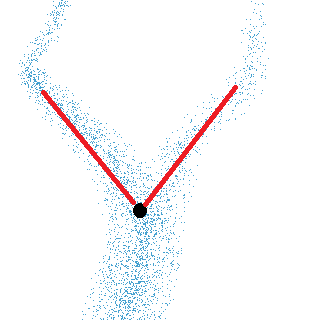
\includegraphics[height=5cm]{branch.png}
	\caption{线性拟合计算分支方向}
	\label{fig:fitting}
\end{figure}

算法\ref{alg:sklextract}给出了得到邻域信息后进行骨架方向抽取的伪代码,其中\textit{Least Squares Processing}表示运用最小二乘法进行
线性拟合。

\begin{algorithm}[H]
	\caption{基于邻域的骨架方向计算}
	\label{alg:sklextract}
	\begin{algorithmic}[1] 
		\Require 当前节点体素$V$
		\Require 骨架方向数组$\mathbb{D}[1..n]$
		\Ensure 当前节点子节点集合$\mathbb{S}$
		\ForAll{骨架方向$d\in D$}
			\State $NewChild\gets Least Squares Processing$
			\State $\mathbb{S}.AddChild(NewChild)$
		\EndFor
		\State \Return $\mathbb{S}$
	\end{algorithmic}
\end{algorithm}

\section{拟合子枝长度和半径}
树木骨架的长度和半径对树木模型的真实感有着十分显著的贡献,所以尽可能准确的获得子枝的长度和
半径信息能够有助于重建出极具真实感的树木模型。对于树木枝干半径的获取方法有许多,
主要分为根据规则生成半径和从树木点云结构中获取半径两种方式。

对于基于规则来生成半径,最简单的方法是对树木半径进行线性地递减,即$r=cR$,其中
$r$为子枝半径,$R$是父枝半径,$c$为一个线性倍数,这个倍数可以固定,也可以进行
随机的扰动从而增进多样性。Leonardo da Vinci在经过大量观察后总结出了一种更符合自然规律
的树木父子枝直径的关系公式:$D^2=\sum_{i=1}^n{d_i^2}$,其中$D$为父枝直径,$d_i$为第
$i$个子枝的直径,$n$为子枝的数量。这个公式被广泛地用于树木枝干的半径模拟。

区别于基于规则的半径生成方法,本文为了进一步提升真实感,选择在进行子枝方向抽取的同时,
同样进行半径抽取的方法。注意,用该方法的前提是点云分布须均匀化,然而基于图像进行三维重建
得到的树木点云会呈现表皮化的现象,这是由于图片上的点都是树木的表皮点,所以在得到
三维点云后,是需要进行一些修复工作的,本文用随机点填充的方法对该点云模型进行了实心化
的修复。当点云分布满足均匀化时,在对某个骨架进行拟合之后,对于拟合出来的直线,根据点
到直线的距离,可以同样根据最小二乘法拟合出骨架的半径。
该算法的伪代码在算法\ref{alg:radius}中给出。\\

\begin{algorithm}[H]
	\caption{半径拟合算法}
	\label{alg:radius}
	\begin{algorithmic}[1] 
		\Require 拟合出的当前子枝所在直线$L$
		\Require 当前子枝的点集$\mathbb{S}$
		\Ensure 当前子枝半径$R$
		\State 初始化点到直线距离数组$\mathbb{D}[1,..,n]$
		\For{$i$ = 1 \textbf{to} $n$}
		\State 点到直线距离$\mathbb{D}[i]=CalculateDistance(P, L)$
		\EndFor
		\State 拟合出使得下面式子达到最小值的半径$R$:\[ \sum_{i=1}^n (2\times \mathbb{D}[i] - R)^2  \]
		\State \Return $R$
	\end{algorithmic}
\end{algorithm}

图\ref{fig:radius}给出了三种半径求解方法的效果对比。\ref{fig:radius}(a)给出了线性衰减方法
的结果,该方法中子枝半径以父枝半径的线性倍衰减。\ref{fig:radius}(b)给出了前文提到的Leonardo
 da Vinci规则所生成的半径情况。\ref{fig:radius}(c)则采用本文中基于线性拟合的方法。
 从三者的效果中可以看出,线性衰减容易出现部分枝条生长不自然的现象,究其
 原因,还是因为一个单一的绝对的线性系数无法适用于所有的枝条,它对于某些枝条会偏大,对于另外一些
 枝条会偏小。 Leonardo规则虽然给出的是一种父子枝之间的相对关系,从一定程度上解决了线性系数单一
 绝对而导致的问题,但是它生成的树木枝干会出现过于均与化,而没有捕捉到现实中树木各个局部的特征。
 本文的方法则由于其基于对所有点的实际恢复坐标进行统计,而更加注重树木的实际局部特征情况,
 其效果也是三者之中最好的。
 \begin{figure}[H]
	\centering
	\subfloat[样本图像]{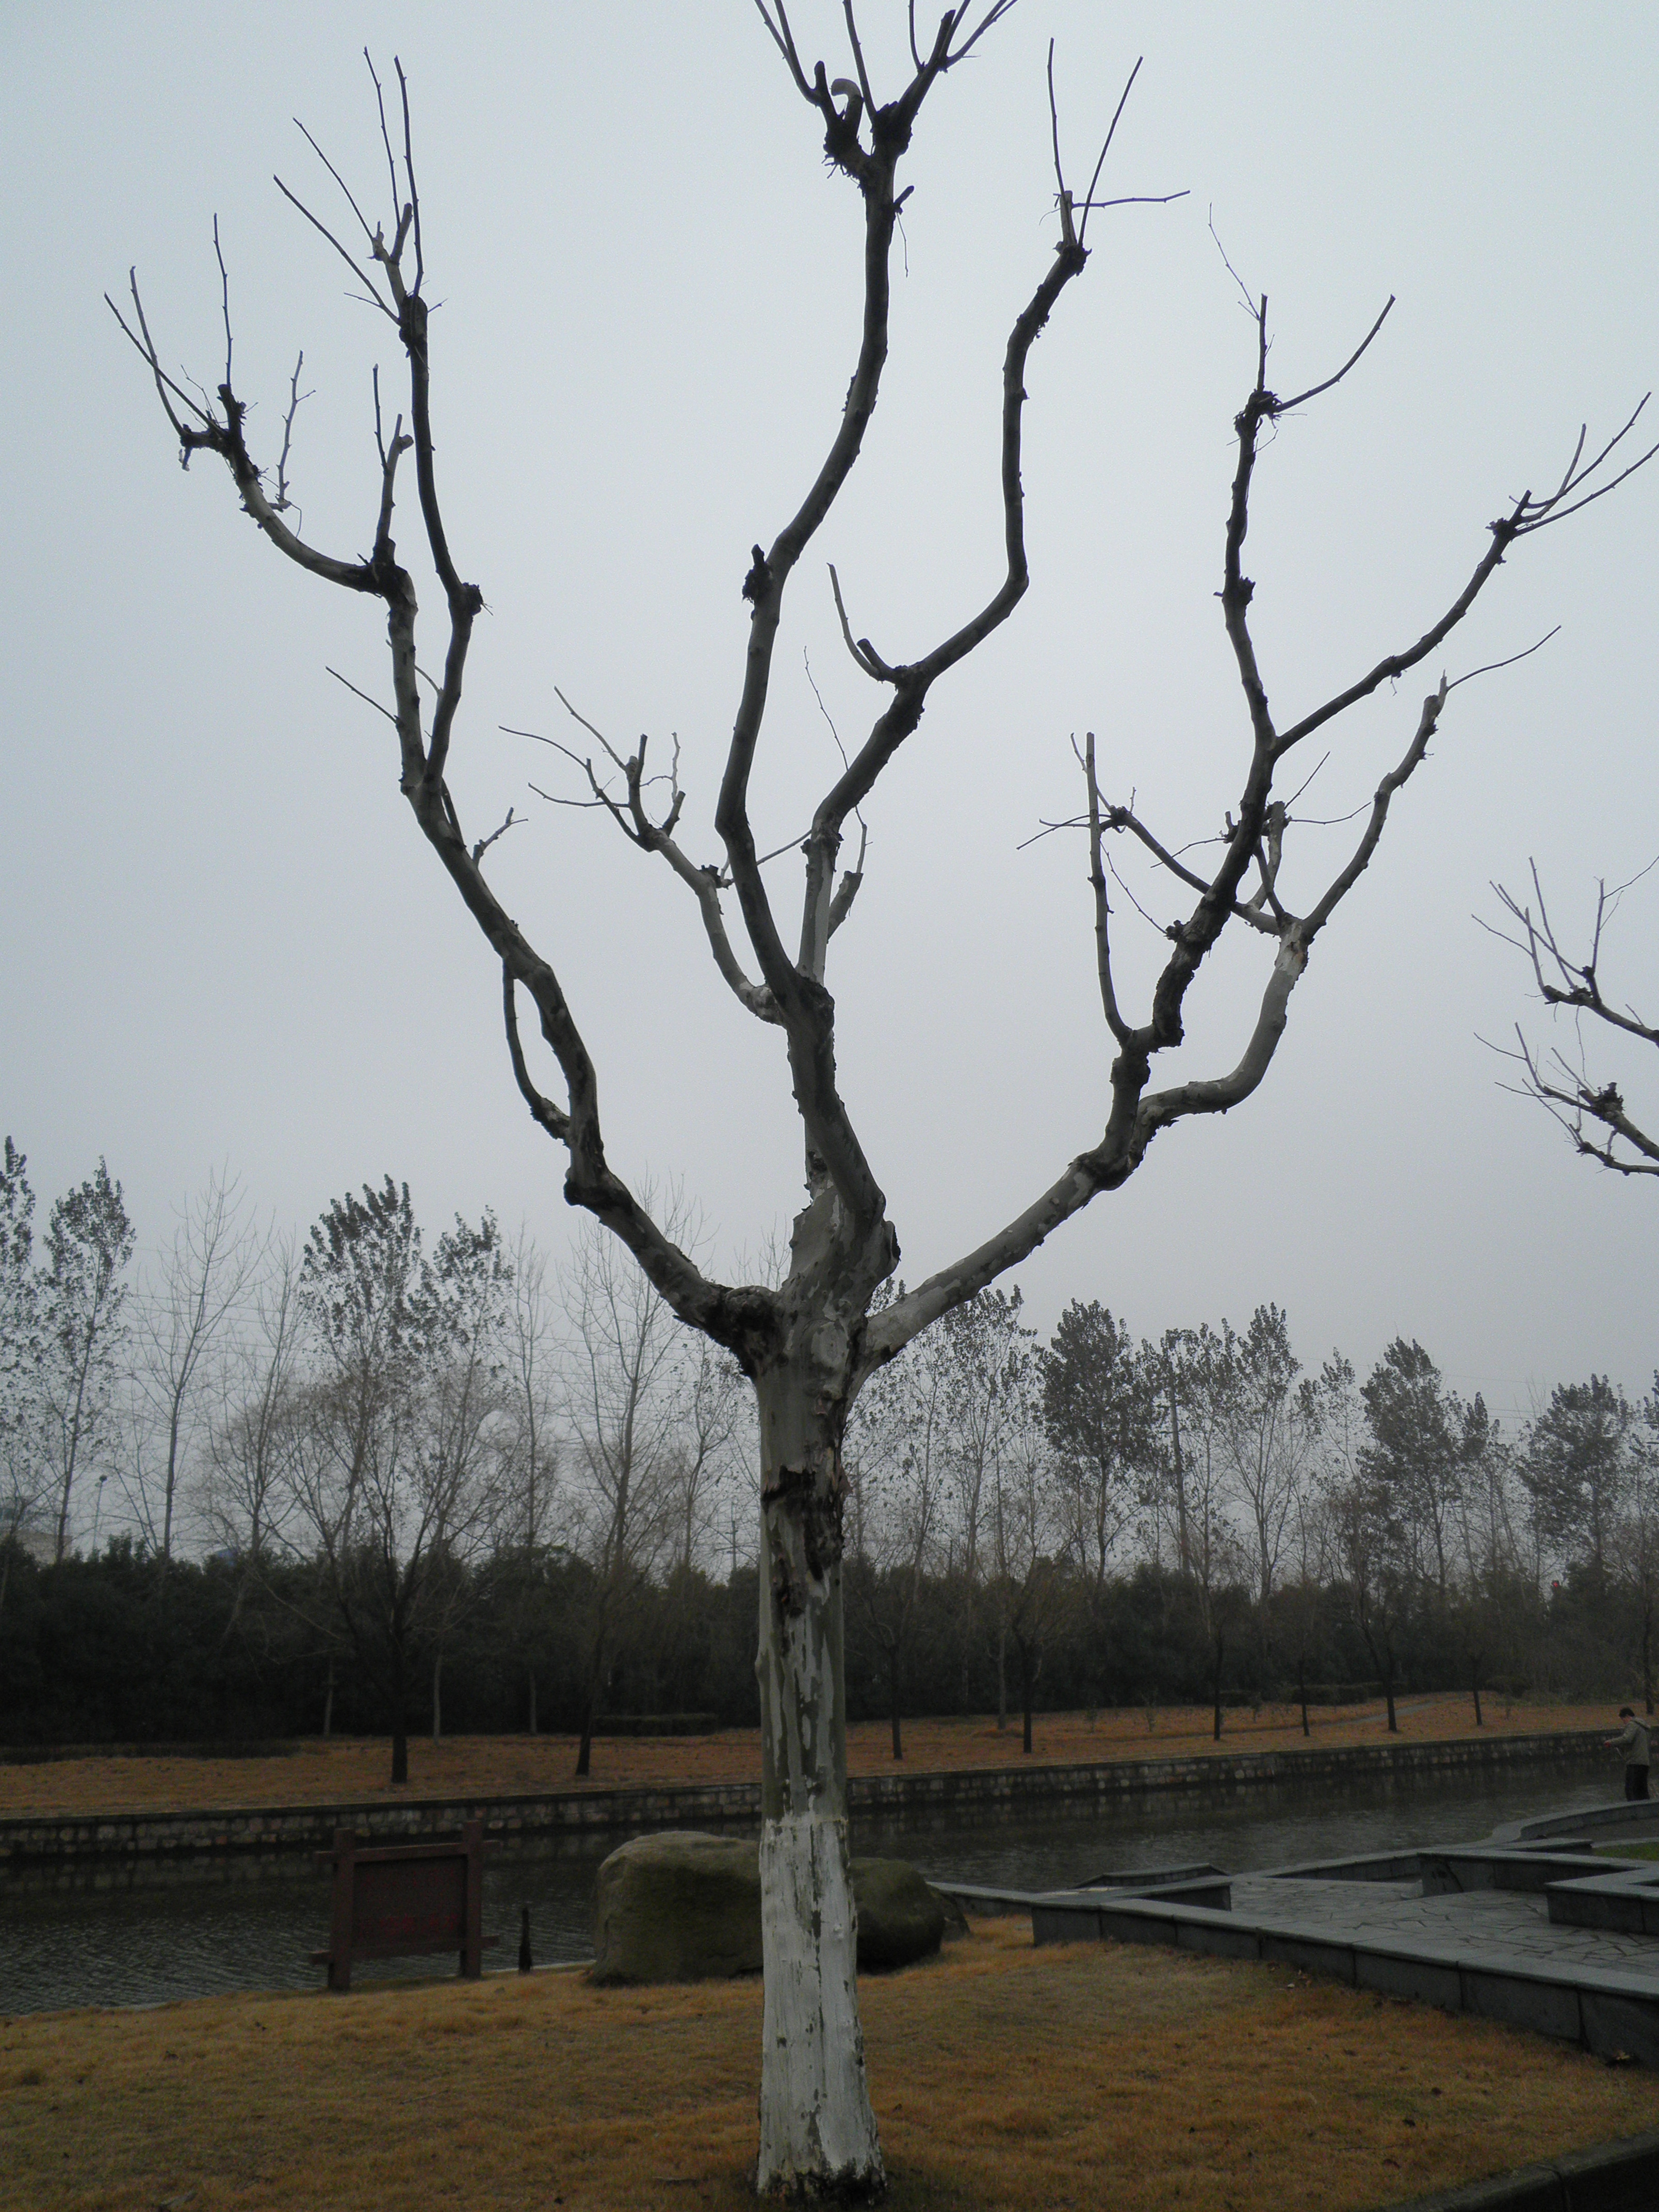
\includegraphics[height=6cm]{rsample.jpg}}\hspace{4em}
	\subfloat[线性衰减(线性衰减系数为0.6)]{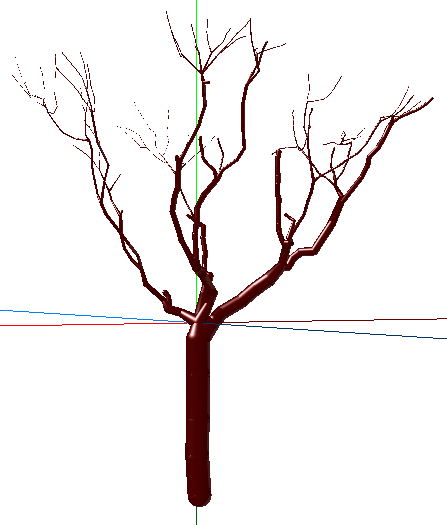
\includegraphics[height=6cm]{rlinear.png}}\hspace{4em}
	\subfloat[Leonardo规则生成($D^2=\sum_{i=1}^n{d_i^2}$)]{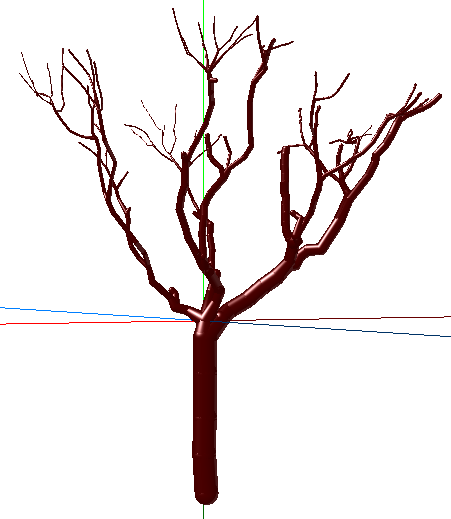
\includegraphics[height=6cm]{rsquare.png}}\hspace{4em}
	\subfloat[基于拟合的半径抽取]{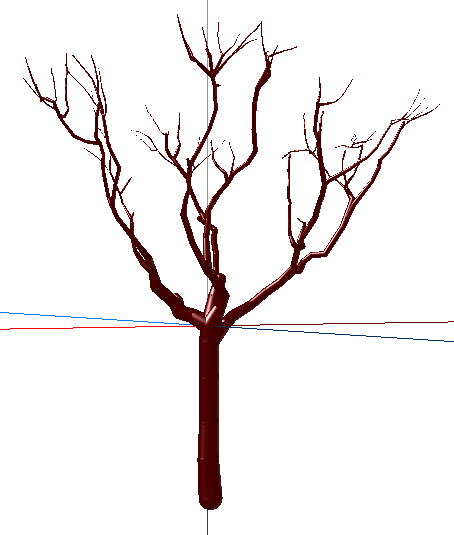
\includegraphics[height=6cm]{raffine.png}}\hspace{4em}
	\caption{三种计算半径方法效果对比}
	\label{fig:radius}
\end{figure}

对于骨架长度的估计,基于规则的生成则并不那么具有实践性,因为树木枝干的长度往往并不像半径那样
随着父子关系而递减。相反地,它地规则往往要复杂许多,而且并没有统一的规则。基于此考虑,本文并
没有对基于规则的长度估计进行实践,而是直接用与半径类似的方法,根据已拟合出的直线,试图从统计
的角度对其枝条长度做出合理的估计。一个直观而可行的方法,是将当前节点与所有该方向邻域的点的连线向量
投影到拟合出的直线方向向量上,然后根据拟合的方法得到高精确度的长度信息。
子枝长度拟合的伪代码,列在了算法\ref{alg:length}中。

\begin{algorithm}[H]
	\caption{子枝长度拟合算法}
	\label{alg:length}
	\begin{algorithmic}[1] 
		\Require 拟合出的当前子枝方向向量$L$,父节点$N$
		\Require 当前子枝的点集$\mathbb{S}$
		\Ensure 当前子枝长度$l$
		\State 初始化父节点到邻域点的向量投影长度数组$\mathbb{D}[1,..,n]$
		\For{$i$ = 1 \textbf{to} $n$}
		\State 父节点到$\mathbb{S}[i]$的向量$Dir=\mathbb{S}[i]$.Position-$N$.Position
		\State $Dir$在$L$上的投影距离$\mathbb{D}[i]$ = CalculateProjectionLength$(Dir, L)$
		\EndFor
		\State 拟合出使得下面式子达到最小值的长度$l$:\[ \sum_{i=1}^n (2\times \mathbb{D}[i] - l)^2  \]
		\State \Return $l$
	\end{algorithmic}
\end{algorithm}

\section{本章小节}

本章首先将三维重建得到的点云数据进行体素化,通过对体素求解包围盒、空间分块、点云索引的方法,将离散的点云数据
转化为连续的体素数据。

接着本章提出了基于新的树木骨架抽取方法,主要包含:\\
\begin{itemize}
	\item \textbf{多种子点的并发三维体素泛洪}: 该方法通过广度优先的方法,对树木节点进行遍历。同时对于同一层级
		上的节点,将它们作为种子点,并并发的进行三维体素的泛洪,以将节点间的相互影响降至最低。
	\item \textbf{最小二乘法拟合骨架信息}: 该方法通过最小二乘的方法,对空间的局部点云进行方向、半径和长度的
		拟合,从而以统计的方法从大量的空间点数据中抽取出有用的骨架信息。
\end{itemize}

通过本章的方法抽取出的骨架具有很高的准确性和真实感,因为它是通过统计的方法在实际的点云中进行信息的获取,相比
起其他的基于规则的信息抽取方法,该方法有明显的优势。
